\section{Description}

This is a lab report of the second given mandatory assignment in control systems engineering 2022. The assignment is answered by students at NTNU Ålesund, November 2022.

A servo motor is connected to a balance beam via a pole. Adjusting the servo position will change the angle, $\alpha$, between the horizontal plane and the balance beam. An IR-sensor connected to a Arduino micro controller is used to measure the distance to a rolling ball on the balance-beam. The goal is to make the ball stay at a predetermined position on the balance beam by regulating the servo-position and thereby the angle of the balance-beam. Under you can see a full list of given values and variables as well as a 3D rendered model of the system.
\vfill

All given values and variables of the system:


\begin{tabular}{ll}
Beam length:                           & L = 0.4m\\
Disc radius:                           & d = 0.06m\\
Angel between lever arm and disc:      & $\theta$\\
Distance between ball and sensor:      & 0.1m $\leq$ r $\leq$ 0.3m\\
Diameter of ball:                      & R = 0.04m\\
Angel between lever and beam:          & $\beta$\\
Height of lever arm:                   & h = 0.09m\\
Angel between beam and bottom plate:   & $\alpha$\\
\end{tabular}                                   


\begin{figure}[h]
    \centering
    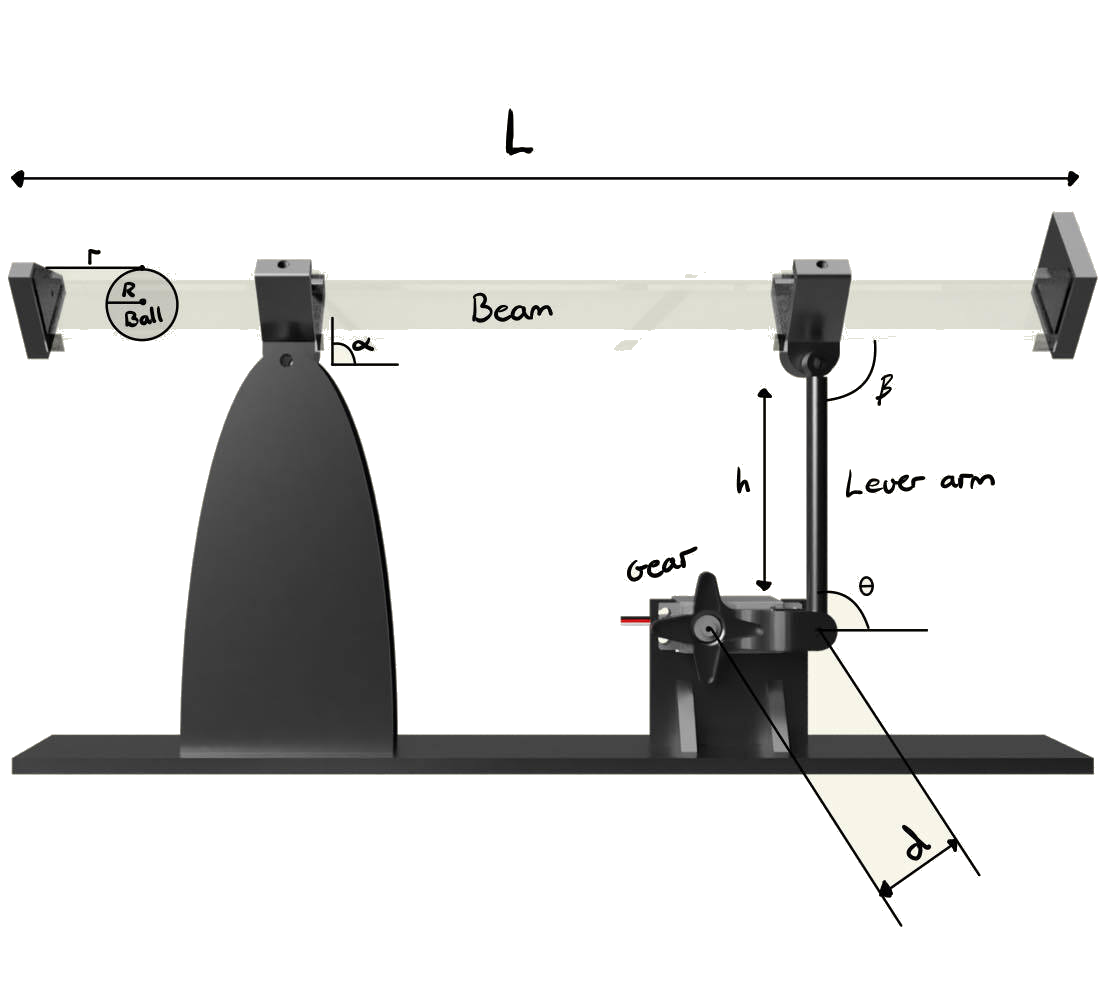
\includegraphics[width = 1\textwidth]{Code/Images/3D-MAIN.png}
    \caption{3D rendered model of the physical system with given variables}
    \label{fig:3d-model}
\end{figure}

